\documentclass[a4paper, 11pt, oneside]{book}
\parindent0pt  \parskip10pt
\usepackage[margin=0.5in]{geometry}

\usepackage{amsmath}

\usepackage{setspace}
\newcommand\epigraph[3]{
\vspace{1em}\hfill{}\begin{minipage}{#1}{\begin{spacing}{0.9}
\small\noindent\textit{#2}\end{spacing}
\vspace{1em}
\hfill{}{#3}}\vspace{2em}
\end{minipage}}

\usepackage{graphicx}
\usepackage{afterpage}

\usepackage{fancyhdr}
\mainmatter
\pagenumbering{arabic}
\pagestyle{fancy}
\fancyhf{}
\renewcommand{\headrulewidth}{0.5pt}
\renewcommand{\footrulewidth}{0pt}
\addtolength{\headheight}{1.6pt}
\fancypagestyle{plain}{}

\setlength{\parindent}{5ex}
\setlength{\parskip}{1em}
\usepackage{indentfirst}

\author{Igor Uspeniev}
\title{%
	Entropy of Implicit Functions \\~\\
	\large Deep Learning Dataset Reproduction Formed by Unknown Smooth \\
	Implicit Functions of Arbitrary Complexity}
\date{April 2019}

\begin{document}
	
\maketitle

\tableofcontents
\thispagestyle{empty} 
      
%=====================================
\chapter*{Abstract}
\addcontentsline{toc}{chapter}{Abstract}
\thispagestyle{empty}
This paper is devoted to measuring the entropy of smooth implicit functions and exact reproduction of their probability distribution through multidimensional numerical arrays without using a priori models. For observable characteristics of an object or a process, a probability distribution is formed for the desired values combination. The error is limited only by computational resources, the accuracy of the original measurements and the representativeness of the sample.

However, the reproduction of an unknown implicit function as a parametric mapping operator does not occur, and the concept of an equation of implicit function does not arise. This is possible due to the indirect measurement of the space dimensions in which the uncertainty of an unknown interdependency reaches equilibrium by the values of its manifestations. The iterative build-up of the dimension of the spatial representation works consistently and inexorably, fixing hidden patterns of arbitrary type and complexity.
\afterpage{\cfoot{\thepage}}

%=====================================
\chapter{Glossary}
\pagestyle{fancy}
\fancyhf{}
\lhead{\bfseries\leftmark}
\rhead{\bfseries\rightmark}
\fancyfoot{}
\fancyfoot[R]{\thepage}
\begin{tabular}{r l}
 $N$ & set of natural numbers \\ 
 $Z$ & set if integer numbers \\  
 $R$ & set of real numbers \\
 $C$ & set of complex numbers \\
 $Re(x)$ & real part of complex number $x$ \\
 $Im(x)$ & imaginary part of complex number $x$ \\
 \big[$a$, $b$\big] & closed interval between $a$ and $b$ \\
 $a \in A$ & $a$ is an element of the set $A$ \\
 $A=\{a, b, c\}$ & set $A$ consists of $a$, $b$ and $c$ \\
 $A \subset B$ & subset: every element of $A$ is also element of $B$. But $A \neq B$ \\
 $A \subseteq B$ & subset: every element of $A$ is also element of $B$. Sets can be equal \\
 $A = B \cup C$ & set $A$ if equal to the union of sets $B$ and $C$ \\
 $\{x_i\}$ & set of elements $x_i$ \\
 $(a_0, b_0)$ & point with coordinates $a_0, b_0$ \\
 $\{(a_i, b_i): \ldots \}$ & a set of elements, each of which consists of values $(a_i, b_i)$ with conditions $\ldots$ \\
 $U(x_0)$ & neighbourhood of point $x_0$ \\
 $U(x_0, \varepsilon)$ & $\varepsilon$-neighbourhood of point $x_0$ \\
 $\exists v, \ldots$ & there is at least one $v$ such that $\ldots$ \\
 $\forall v$ & for every $v$ \\
 $v = f(t)$ & variable $v$ is a function of a variable $t$ \\
 $f(t, v, g, u)$ & function of several variables: $t, v, g, u$ \\
 $u(t_0)$ & value of function $u(t)$ in the point $t_0$ \\
 $g(u(t))$ & complex function of argument $t$, composition of functions $y = u(t)$ and $g(y)$ \\
 $i = m, \ldots, n$ & integer number $i$ takes sequentially all values from from $m$ to $n$ inclusively \\
 $\sum\limits_{i=m}^n d_i$ & sum of $n - m + 1$ elements: $d_m, d_{m+1}, \ldots, d_i, \ldots, d_{n-1}, d_n$ \\
 $t \to b$ & variable $t$ tends to $b$ \\
 $f(x) =
 \begin{cases}
  a: & ...\\
  b: & ...
 \end{cases}$ & function $f(x)$ takes value $a$ on condition $\ldots$ , and takes value $b$ on condition $\ldots$ \\
 $\partial t$ & differential of argument $t$ \\
 $\frac{\partial v}{\partial t}, v', v_t'$ & Derivative of function $v$ \\
 $v^{(n)}$ & derivative of function $v$ of order $n$ \\
 $a^b$ & exponentiation with base $a$ and the exponent of power $b$ \\
 $ln a$ & natural logarithm of variable $a$ (logarithm to the base of the constant $e$) \\
 $log_{a} b$ & logarithm of variable $b$ to the base of $a$ \\
 $sin(a), cos(a)$ & sine, cosine of variable $a$ \\
 $tan(a), cot(a)$ & tangent, cotangent of variable $a$ \\
 $arcsin(a), arccos(a)$ & arcsine, arccosine of variable $a$ \\
 $arctan(a), arccot(a)$ & arctangent, arccotangent of variable $a$ \\
 $sinh(a), cosh(a)$ & Hyperbolic sine, cosine of variable $a$ \\
 $tanh(a), coth(a)$ & Hyperbolic tangent, cotangent of variable $a$
 
\end{tabular}

%=====================================
\chapter{Base of Reproduction}
\pagestyle{fancy}
\fancyhf{}
\lhead{\bfseries\leftmark}
\rhead{\bfseries\rightmark}
\fancyfoot{}
\fancyfoot[R]{\thepage}

\epigraph{4in}{This method is ineffective because here you need to think. And when a person thinks, he becomes nervous and wrong.}{Vadim Serebryannikov}

\section{Problem Formulation}
\subsection{Models of Generic Properties}
Many tasks of numerical arrays processing are associated with the detection and generalization of properties. In computer vision tasks, this is the identification of features, their tracking and matching. In forecasting tasks, this is the calculation of the deviation of sequences from each other. In general, this is the recovery of hidden patterns and dependencies.

Whether it is inside the computer system or on paper using manual calculations, the generalization and iterative refinement of the generic property in any case requires a formal mathematical description of this property. And this description should have no flexibility restrictions, providing the possibility of data modelling from real life in a full variety of processes. In other words, a mathematical model of a property can potentially contain any combination of polynomials, trigonometry, logarithms, and other conceivable components that describe the observed property nature.

We have a dual task:
\begin{enumerate}
	\item On the one hand, we strive to select a model whose values most closely match the observed values of the actual data.
  \item On the other hand, we strive to minimize the complexity (entropy) of the model, avoiding its retraining and over-calibration for a specific sample.
\end{enumerate}

And here the problem begins. The concept of entropy of a function (including implicit, parametrically defined) does not have a generally accepted quantitative definition. Moreover, there is no known method of complete enumeration of all known functions from simple to complex, making it impossible to explicitly prioritize their consideration - how can we be sure that we did not miss the best option?

Imagine that in a series of photographs a recognizable feature can be described with quite good accuracy by the logarithm of a third-degree polynomial. But we also know that the fractional degree of the arc sine of a quadratic function can be applied. Which of these models to choose and why? A practical experiment with the choice of a more accurate fit of the model to real data can be a judge, but we understand that these two potential models are not the only ones, there are more complex and more precisely fitting functions. And their number is infinite. We need to sort them out from simple to complex - in what sequence will we begin the search and at what stage should we say that further building up the entropy of the function is inappropriate?

To do this, we must quantify the entropy of the implicit function.

The measurable entropy (uncertainty, complexity, information capacity) of the implicit function is the subject of research of this work. We will also consider the principles of the universal definition of an implicit function and the reduction of an arbitrary function to this form. And finally, we will formulate how in machine learning we can detect the characteristic properties using the flexibility of the universal definition.

\subsection{Brief Review of Existing Approaches}
Today, the concept of entropy of an implicit function does not have a generally accepted formal definition. If we consider it from the point of view of the informational entropy of the values of this function, then such an approach is limited to a discrete alphabet of these values \cite{Shannon_book}\relax, and also provides only a general assessment without analysing the patterns, which is considered as a separate task. Selection of a model for a data set is most often carried out in the following ways:
\begin{enumerate}
	\item An a priori choice of a deliberately complex function, the deviation of which from the training dataset can be minimized due to the huge number of parameters \cite{KollerFriedman_book}\relax, \cite{Frydenberg_book}\relax, \cite{RichardsonSpirtes_book}\relax.
  \item Analysis of the subject area of a dataset producer process for a comprehended choice of the mathematical model or its parts approximating the expected dependencies.
\end{enumerate}
These options are effective in some simple approximation, but they have unrecoverable problems:
\begin{enumerate}
	\item The higher the complexity of the dependencies that must be reproduced, the less likely the selection of the optimal model by a prior choice or expert evaluation. As a result, the model does not correspond to the process being analysed, and accuracy inevitably falls. More importantly, the accuracy often becomes unpredictable on when expanding a dataset.
  \item The optimality of the found model and its parameters cannot be analytically justified compared to many alternatives except by deviation from the original data. However, using only one optimization parameter, we inevitably come to an unlimited enumeration of models, the comparison of which, by complexity, has no quantitative justification.
  \item The very determination of a model as a parametric mapping operator cuts off the possibility of reproducing a function as a probability distribution of a flexible form. Or it is issued in the form of an artificially specified and unreasonable distribution.
\end{enumerate}

The more complex the unknown process or object, which generates the analysed dataset, the more difficult the reproducing heuristic model and the lower its accuracy. Only in special cases, it is possible to manually choose a model of the behaviour of the observable quantity in the form that corresponds to an unknown function. The capabilities of the expert are always limited and, starting with a certain level of complexity and entanglement, useful data become indistinguishable from random variables. With this approach, only a well-studied and decomposed process can be successfully modelled and reproduced by a priori models.

Actual automated tools for sorting models in practice are no different in quality from the actions of an expert, only expanding the quantitative variation of selection and depth of nesting.

To build more effective approaches, a universal and fully automatic method of reproducing implicit functions is needed, which is not only describe any of their variants, but be evenly oriented on all of their diversity, without giving preference to the a priori view. The complexity (entropy) of the reproducing tool must be measurable and grow according to the entropy of the incoming data, which is the reason for the task. This paper is dedicated to this goal.

\section{Input Data}
\subsection{Dimension and values}\label{subs:dimension_and_values}
In datasets according to their structure, we can sometimes distinguish the nature of data. In trivial case there are a priori independent values (arguments) and dependent on these argument values (observed values). For example, for a series of photographs, the arguments can be the time moment of photo, the horizontal and vertical coordinates of the pixel, and the observed values can be R, G, and B color characteristics of this pixel (Figure \ref{fig:pixels}).

\begin{figure}[h!]
  \centering
  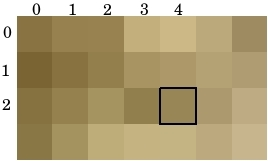
\includegraphics[width=3in]{./anc/figure01.jpg}
  \caption{Bitmap image. Arguments: time moment, coordinates $(x, y)$. Observed values: R, G, B colors.}
  \label{fig:pixels}
\end{figure}

In a slightly more complicated case the range of definition of arguments can be the field of real numbers without the periodic "grid", and the filling with observed values can be non-complete. An example is given in Table \ref{table:tivi}.

\begin{table}[h!]
  \centering
  \begin{tabular}{||c c c c c c c c||}
    \hline
    $t_1$ & $t_2$ & ... & $t_n$ & $v_1$ & $v_2$ & ... & $v_m$ \\ [0.5ex] 
    \hline
    -0.04982123 & 68.04892 & ... & 3.993287 & Unknown & 2.412349E-9 & ... & 7821.397 \\ 
    0.1983995 & 19.95884 & ... & 493.8401 & 15.41245 & Unknown & ... & 8503.325 \\
    0.023891 & 34.984177 & ... & 1085.0193 & 15.41183 & Unknown & ... & 48.00832 \\
    -3.009583 & 18.11842 & ... & 782.3989 & 15.41396 & 8.982384E-10 & ... & -26.38449 \\ [1ex] 
    \hline
  \end{tabular}
  \caption{Example of input data with arguments $t_i$ and observed values $v_i$}
  \label{table:tivi}
\end{table}

However, in the general case, it is impossible to a priori divide the array of source data into independent arguments and dependent values. The values of the dataset are potentially interdependent and none of the dependencies are guaranteed to be surjective mapping, the definition of the multivariable functions is conceivable here only in an implicit form \cite{Cauchy_book}\relax, \cite{Ulisse_book}\relax. All the initial data by default consist only of observable values, the prior selection of independent arguments is the risk of the expert, which is unacceptable with the general approach.

Even those quantities that seem independent can appear as computable. For example, in the image, pixel coordinates of the observed objects may be the result of counting third-party entities that are not at all observable in the image, in this case we do not observe truly independent arguments, and their indirect determination is an inevitable task of finding hidden patterns.

Thus, in the general case, the array of input data consists solely of the observed values:

\begin{table}[h!]
  \centering
  \begin{tabular}{||c c c c c c c c||}
    \hline
    $v_1$ & $v_1$ & ... & $v_n$ & $v_{n + 1}$ & $v_{n + 2}$ & ... & $v_{n + m}$ \\ [0.5ex] 
    \hline
    -0.04982123 & 68.04892 & ... & 3.993287 & Unknown & 2.412349E-9 & ... & 7821.397 \\ 
    0.1983995 & 19.95884 & ... & 493.8401 & 15.41245 & Unknown & ... & 8503.325 \\
    0.023891 & 34.984177 & ... & 1085.0193 & 15.41183 & Unknown & ... & 48.00832 \\
    -3.009583 & 18.11842 & ... & 782.3989 & 15.41396 & 8.982384E-10 & ... & -26.38449 \\ [1ex] 
    \hline
  \end{tabular}
  \caption{Example of input data by regular default}
  \label{table:vi}
\end{table}

On the basis of these prerequisites, we will build the logic of finding patterns and generalizing properties.

\subsection{Two-Dimensional Case}\label{subs:trivial-case}
For a consistent presentation of the theory from simple to complex, we begin the consideration with a two-dimensional dataset and an a priori surjective relationship formed by an unknown function $v=f(t)$, where one scalar argument $t \in C$ corresponds to one scalar observed value $v \in C$. Thus, let's consider an input dataset:
\begin{equation}\label{eq:2-dim-dataset}
  \Omega_k = \{(t_i, v_i)\}: i \in [1, k], \{i, k\} \in N
\end{equation}

The power of the set may be infinite, but the practically analysed number of elements is always limited. The observed value can be:
\begin{itemize}
  \item The value of the unknown source function $v = f(t)$,
  \item The value of the numerical property $v$ of conditionally closed physical system. Change the given numerical property in accordance with the value $t$ can also be represented as an unknown source function $v = f(t)$
\end{itemize}
When analysing the dataset, the following objectives are possible:
\begin{itemize}
  \item Prediction or recovery of lost values,
  \item Noise removal, detection of errors and correction of incorrectly measured values,
  \item Identifying similar characteristics at intervals.
\end{itemize}

Such goals are often attempted to be achieved by constructing a model of the unknown function, but it is important to understand that a model is never the ultimate goal, but only a means to achieve this goal. Therefore, if the result can be obtained without defining the model of the unknown function, this will be a successful solution to the problem.
Such goals are often attempted to be achieved by constructing a model of the desired function, but it is important to understand that strictly speaking a model as a mapping operator is never the ultimate goal, but only a possible instrument of achieving this goal. Therefore, if the result can be obtained without defining such a model, then this will be a successful solution to the problem. The ultimate goal is the reproducing values of an unknown function.

Consideration the unknown function $v = f(t)$ by its manifestations $\Omega_k$ can be conducted using the set of reproducing functions $\{m_j(t)\}$ passing through this dataset. The probabilistic criterion for the reproducing function applicability with respect to the given data is the deviation between reproducible $m_j(t_i)$ and actual values $v_i$ corresponding to the same $t_i$:
\begin{equation}\label{eq:deviation-of-2d-dataset}
  \Theta(m_j, \Omega_k) = D(\{(t_i, m_j(t_i), v_i)\}): i \in [1, k], \{i, k\} \in N
\end{equation}

In trivial case the error estimation function can be based on the standard deviation or other means of numerical aggregation and normalised to $[0, 1]$ as probability domain. For example using mean square error metric we get following quantitative criterion of function $m_j(t)$ applicability:
\begin{equation}\label{eq:MSE-of-2d-dataset}
  \Theta(m_j, \Omega_k) = 1 - \frac{1}{1 + e^{\displaystyle -\frac{1}{k} \sum_{i = 1}^k (m_j(t_i) - v_i)^2}}
\end{equation}

To keep only implying reproducing functions whose deviation is not too large, we can optionally apply the constraint:
\begin{equation}\label{eq:acceptable-deviation-of-2d-dataset}
  {m_j(t)}: \Theta(m_j, \Omega_k) \geq \gamma
\end{equation}

Integrating the sheaf of reproducing functions with regard to their quantitative applicability criterion, we obtain the complete model of the unknown function in the form of its probability density:
\begin{equation}\label{eq:full_model-for-2d-dataset}
  g(t, v, \Omega_k) = \frac{\displaystyle \sum_{j = 0}^{\infty} \Big((P(m_j(t) \leq v) \cdot \Theta(m_j, \Omega_k) \Big)}{\displaystyle \sum_{j = 0}^{\infty}\Theta(m_j, \Omega_k)}: P(x) = \begin{cases}1: x = true\\0: x = false \end{cases}
\end{equation}

This approach is theoretically correct, but practically useless, since even using \ref{eq:acceptable-deviation-of-2d-dataset} with $\gamma = 1$ the set $\{m_j(t)\}$ will still contain an infinite number of reproducing functions passing through a finite number of points in the dataset $\Omega_k$. It is impossible to generate and take into account all this variety of functions of arbitrary complexity. Respectively the total probability distribution of the unknown function cannot be calculated in this way.

Assume some set of probabilistic sheaf of $\mu_i$ functions represented in the form of an unnormalized density \ref{eq:function-aggregation-into-sheaf} that can be with high accuracy replaced by an analytically formulated distribution $w_i(t, v, \Omega_k)$.
\begin{equation}\label{eq:function-aggregation-into-sheaf}
  \frac{1}{\mu_i} \sum_{j = 0}^{\mu_i} \Big((P(m_j(t) \leq v) \cdot \Theta(m_j, \Omega_k) \Big): P(x) =
  \begin{cases}
    1: x = true\\
    0: x = false
  \end{cases} \\
\end{equation}

For the sake of brevity let's call such analytically formulated distribution $w_i(t)$ as f-pattern. If there is a pretty accurate representation method of an infinite number of reproducing functions $\{m_j(t)\}$ as a finite set of f-patterns $\{w_i(t, v, \Omega_k)\}$ then full model \ref{eq:full_model-for-2d-dataset} calculation would be practically applicable. In this case, the probability density of the unknown function $v=f(t)$ based on these f-patterns will be equal to:
\begin{equation}\label{eq:full_model-for-2d-dataset-by-f-patterns}
  g(t, v, \Omega_k) = \frac{\displaystyle \sum_{i = 0}^p w_i(t, v, \Omega_k)}{\displaystyle \lim_{\sigma \to \infty}\sum_{i = 0}^p w_i(t, \sigma, \Omega_k)}
\end{equation}

Such grouping of f-patterns is possible only if there is a method of aggregation of functions to f-pattern and an analytical description of such f-patterns, as well as the possibility of ranking f-patterns by measurable complexity (entropy), so that the least f-patterns templates can be neglected. However, before we proceed to the sequential recovery of these patterns, let's generalize the above definitions to the multidimensional case.

\subsection{Multidimensional Case}
Let us generalize formulas and definitions from subsection \ref{subs:trivial-case} to the case with higher dimensions from subsection \ref{subs:dimension_and_values}. The initial data array is a set of elements, each of which is a vector of mutually corresponding observed values:
\begin{align}\label{eq:nd-dataset}
  \begin{split}
    \Omega_k = \{(v_{1, i}, v_{2, i}, \ldots, v_{\psi, i})\}: i \in [1, k], \{i, k, \psi\} \in N
  \end{split}
\end{align}

Due to potentially implicit form of functional interdependencies between observed values $v_{q, i}: q \in [1, \psi]$ we have the set of unknown functions $v_q = f_q(T): q \in [1, \psi]$ based of vector $T$ of unobservable variables. Consideration these unknown functions by their manifestations $\Omega_k$ can be conducted using the $\psi$ separate sets of reproducing functions $\{m_{psi, j}(T)\}$ passing through corresponding $v_{q, i}: q \in [1, \psi]$ values of this dataset. The probabilistic criterion for the reproducing functions applicability with respect to the given data is based on the deviation between reproducible $m_{\psi, j}(T_i)$ and actual values $v_{\psi, i}$ corresponding to the same $T_i$ that also needs to be recovered:
\begin{equation}\label{eq:deviation-of-nd-dataset}
  \Theta(m_{q, j}, \Omega_k) = D(\{(T_i, m_{q, j}(T_i), v_{q, i})\}):
  \begin{cases}
    i \in [1, k] \\
    q \in [1, \psi]
  \end{cases}
\end{equation}

To keep only implying reproducing functions whose deviation is not too large, we can optionally apply the constraint:
\begin{equation}\label{eq:acceptable-deviation-of-nd-dataset}
  {m_{q, j}(t)}: \Theta(m_{q, j}, \Omega_k) \geq \gamma
\end{equation}

Integrating the sheaf of reproducing functions with regard to their quantitative applicability criterion, we obtain the \textbf{complete model} of the unknown function in the form of its probability density:
\begin{equation}\label{eq:full_model-for-nd-dataset}
  g(T, v_q, \Omega_k) = \frac{\displaystyle \sum_{j = 0}^{\infty} \Big((P(m_{q, j}(T) \leq v_q) \cdot \Theta(m_{q, j}, \Omega_k) \Big)}{\displaystyle \sum_{j = 0}^{\infty}\Theta(m_{q, j}, \Omega_k)}:
  \begin{cases}
    P(x) = \begin{cases}1: x = true\\0: x = false \end{cases} \\
    q \in [1, \psi]
  \end{cases}    
\end{equation}

Analogically with two-dimensional case, assume some set of probabilistic sheaf of $\mu_{q, i}$ functions in the form of an unnormalized density \ref{eq:n-functions-aggregation-into-sheaf} that can be with high accuracy replaced by an analytically formulated f-pattern $w_{q, i}(T, v_q, \Omega_k)$.
\begin{equation}\label{eq:n-functions-aggregation-into-sheaf}
  \frac{1}{\mu_{q, i}} \sum_{j = 0}^{\mu_{q, i}} \Big((P(m_{q, j}(t) \leq v) \cdot \Theta(m_{q, j}, \Omega_k) \Big):
  \begin{cases}
    P(x) =
    \begin{cases}
      1: x = true\\
      0: x = false
    \end{cases} \\
    q \in [1, \psi]
  \end{cases}
\end{equation}

If there is a pretty accurate representation method of an infinite number of reproducing functions $\{m_{q, i}(T)\}$ as a finite set of f-patterns $\{w_{q, i}(T, v_q, \Omega_k)\}$ then full model \ref{eq:full_model-for-nd-dataset} calculation would be practically applicable. In this case, the probability density of the unknown function $v=f(T)$ based on these f-patterns will be equal to:
\begin{equation}\label{eq:full_model-for-nd-dataset-by-f-patterns}
  g(t, v_q, \Omega_k) = \frac{\displaystyle \sum_{i = 0}^p w_{q, i}(t, v_q, \Omega_k)}{\displaystyle \lim_{\sigma \to \infty}\sum_{i = 0}^p w_{q, i}(t, \sigma, \Omega_k)}
\end{equation}

As in two-dimensional case such grouping of f-patterns is possible only if there is a method of aggregation of functions to f-pattern and an analytical description of such f-patterns, as well as the possibility of ranking f-patterns by measurable complexity (entropy), so that the least f-patterns templates can be neglected. Accordingly, it is also necessary to determine the metric of functional entropy. To do this, we will consider a few definitions, and then generalize them to an algebraic description.

\section{Logic of Entropy}
\subsection{Axiom of the Reproduction Supportability of the Unknown Function}\label{subs:axiom-of-the-reproduction}
Reproduction of unknown function should be determined strictly by the dataset formed by the unknowns functions. Neither the type of reproduction models, nor their parameters can be set a priori or randomly.

In the absence of this axiom, a causal relationship between the condition and the solution cannot be built, and the criteria for optimality of the solution cannot be not only proved, but even considered.

On this axiom, all subsequent logic of reasoning in the theory of entropy definition from discrete observations is built. Let's prove a series of statements that are consequences of the axiom of the reproduction supportability of the unknown function.

\subsection{Value of Entropy}
Let's introduce the definition of the function entropy:

The entropy of a function or process is a number evaluating a measure of the information capacity (uncertainty) of the behaviour of this function or process.

The higher the information capacity of the function behaviour, the higher the numerical value of its entropy. Consequently, the constant has the smallest entropy, which is constant in time, and the true random function has the greatest entropy, whose information capacity is infinite


\subsection{Maximum entropy of reproducing functions}\label{subs:maximum-entropy-limit}
The maximum entropy of reproducing functions is determined by the number of elements in the dataset.

\textbf{Proof.}
Since according to the axiom of the reproduction supportability \ref{subs:axiom-of-the-reproduction}, the reproducing functions are determined by the dataset, then the entropy of the reproducing functions is determined by the dataset. At the same time, the amount of information, contained in the set of elements of the dataset is limited by the power of this set. Consequently, the maximum entropy of the reproducing functions is determined by the number of elements in the dataset. Otherwise, the reproducing functions are unreasonable.

Therefore, the number of elements in the dataset determines the maximum entropy of reproducing functions.

\subsection{Minimum entropy of reproducing function}\label{subs:minimum-entropy-limit}
The minimum entropy of the most implying reproducing functions is determined by the values of elements in the dataset.

\textbf{Proof.}
By the definition of a complete model of unknown function \ref{eq:full_model-for-nd-dataset-by-f-patterns}, the smaller deviation , the more imply the reproducing function has. Consequently, the entropy, which determines the degree of freedom of the reproducing function, must be sufficient for the minimizing of deviation.

Therefore, the values of elements in the dataset determines the minimum entropy of the most implying reproducing functions.

\subsection{Increase entropy of reproducing functions}
While the entropy of the reproducing functions is lower than the entropy of the unknown function, an increase in the number of elements of a dataset leads to an increased or unchanged average entropy of implying reproducing functions that satisfy this dataset.

\textbf{Proof.}
Let's consider the input dataset:
\begin{align}\label{eq:increase-entropy-input-omegak}
  \Omega_k = \{(v_{1, i}, v_{2, i}, \ldots, v_{\psi, i})\}: i \in [1, k], \{i, k\} \in N
\end{align}

Assume that there is a set of implying functions $M_n = \{m_{q, j}(T): q \in [1, \psi]\}$ that satisfies acceptable deviation \ref{eq:acceptable-deviation-of-nd-dataset}. Entropy $E_{q, j}$ each of them belongs to closed interval defined by minimum degree of freedom (according to subsection \ref{subs:minimum-entropy-limit}) and set cardinality (according to subsection \ref{subs:maximum-entropy-limit}).

In case of removing one element by random index from the dataset $\Omega_k$ we will get the dataset $\Omega_{k - 1}$:
\begin{align}\label{eq:increase-entropy-input-omegakplus1}
  \Omega_{k - 1} = \{(v_{1, i}, v_{2, i}, \ldots, v_{\psi, i})\}: i \in [1, k - 1], \{i, k\} \in N
\end{align}

To this dataset will satisfy by acceptable deviation filtering the another set of implying functions $M_{n - 1} = \{\widetilde{m_{q, j}}(T): q \in [1, \psi]\}$

These sets can be decomposed as:
\begin{align}\label{eq:increase-entropy-set-unions}
  \begin{cases}
    M_n = S_{n - 1} \cup Q_n \\
    M_{n - 1} = S_{n - 1} \cup B_{n - 1}
  \end{cases}
\end{align}
where $S_{n - 1}$ is a set of reproducing functions that satisfy both datasets $\Omega_{k - 1}$ and $\Omega_k$, $Q_n$ is a set of reproducing functions with entropy value not allowed for $\Omega_{k - 1}$ due to cardinality limitation (according to the subsection \ref{subs:minimum-entropy-limit}), $B_{n - 1}$ is a set of reproducing functions that not satisfy $\Omega_k$ due to one additional element that gives high deviation. Due to entropy of any function from $Q_n$ is higher than entropy of any function from $B_{n - 1}$ we can see that entropy of any function from $M_n$ is higher or equal to entropy of any function from $M_{n - 1}$.

Therefore, an increase in the number of elements of a dataset leads to an increased or unchanged average entropy of implying reproducing functions that satisfy this dataset.

\subsection{Finiteness of necessary argument}
If the multivariable unknown function $v = f(T)$ is reproducible then there is at least one reproducing function $m_0(T)$ that satisfy acceptable deviation \ref{eq:acceptable-deviation-of-nd-dataset} to obtain which we need a finite number of points in the dataset formed by the unknown function.

\textbf{Proof.}
Let us prove this statement by contradiction: let the function $v = f(T)$ is reproducible but there is no reproducible function $m_0(T)$ that satisfies acceptable deviation \ref{eq:acceptable-deviation-of-nd-dataset} and can be obtained using a finite number of points in the dataset formed by unknown function.

Assume that for all $k$ the dataset $\Omega_k$ for which the set of reproducing functions that satisfies the acceptable deviation \ref{eq:acceptable-deviation-of-nd-dataset} doesn't contain any function that satisfy the acceptable deviation for dataset $\Omega_{k + 1}$ that contains additional point of unknown function. Therefore the entropy of reproducing function for $\Omega_k$ will be maximum allowed for $k$ elements and constantly increase with the growing of dataset. Thus, the minimal entropy of reproducing function will be not limited in the lower bound, so the complexity of all reproducing function will be infinite and unknown function is random that is not reproducible. This indicates that the original contradiction statement is incorrect.

Therefore, if the multivariable unknown function $v = f(T)$ is reproducible then there is at least one reproducing function $m_0(T)$ that satisfy acceptable deviation \ref{eq:acceptable-deviation-of-nd-dataset} to obtain which we need a finite number of points in the dataset formed by the unknown function.

%=====================================
\chapter{Theorem of Universal Form}
\pagestyle{fancy}
\fancyhf{}
\lhead{\bfseries\leftmark}
\rhead{\bfseries\rightmark}
\fancyfoot{}
\fancyfoot[R]{\thepage}

\section{Restrictions}
\subsection{Question of Differentiability}
At present, the diversity of functions cannot be represented as arithmetic operations with elementary functions and their compositions. Consequently, this definition cannot be limited, since, by setting the task to make it possible to reproduce an unknown function, expressed in the form of a dataset, we must maximize the considered set of functions.

At the same time, expanding this set, we inevitably face the question of the method of defining functions. And above all with the question - whether to consider the unknown function differentiable. The answer to this question irreversibly divides the ways to solve the problem.

\subsection{Nondifferentiable function}
Consider a negative or indefinite answer to the question of differentiability.
This way of reasoning is quite uncertain, since the question arises about the method of describing non-differentiable functions, each of which can be very specific, ranging from the simplest variants containing a module in the definition to special definitions for nowhere continuous function like Dirichlet functions.
Nondifferentiable functions do not belong to one group for which special methods of functional analysis have been developed. They are united only by the fact that they do not belong to the group of differentiable functions. At the same time, the denial of the possibility of differentiation does not provide additional theoretical tools for functional analysis, but only eliminates many well-known tools inherent in differentiated functions.

\subsection{Differentiable functions}
Consider a positive answer to the question of differentiability. In this case, the set of functions under consideration using differential equations is significantly wider comparing non-differential view of differentiable functions.
For example, a function defined by a differential equation:
\begin{equation}\label{diff-function-example}
  \frac{\partial u}{\partial \phi} = e^{\displaystyle -\phi^2}
\end{equation}
has the solution in quadrature:
\begin{equation}\label{integral-of-diff-function-example}
  u = \int e^{\displaystyle -\phi^2} \partial \phi + c
\end{equation}
integral of which can not be analytically found. However, it does not interfere with the existence of function $u(\phi)$ and to be a part of representation of unknown function that builds the dataset or to be a part of f-pattern that aggregates reproducing functional distribution. Functions expressed in quadratures like $u(\phi)$ is an infinite set, and integral constructions in them can be more complex.

But there is an immeasurably greater number of functions defined in the form of differential equations that cannot be solved in quadratures. These functions exist only in the form of differential equations without the possibility of reducing them to the form $v = f({t_i})$ in no way.

To quadratures, first-order differential equations with an integrating factor, homogeneous and quasihomogeneous equations, Bernoulli equation, some Riccati equation, and some other specially defined forms can be reduced. Differential equations have a solution in quadratures mostly in the case of a linear representation, and even insignificant heterogeneity leads only to evaluative criteria for the correctness of the solution, as in the Liouville's formula. Known general methods for solving inhomogeneous differential equations do not exist at all, but surjective mapping operators that satisfy these equations objectively exist and can act as unknown functions and f-patterns of reproducing them.
Thus, in the case of an affirmative answer to the question of differentiability, especially with infinite differentiability, we are forced to consider many functions in the form of their differential representation, taking into account the potential impossibility of bringing them to a non-differential form. However, non-differentiable (nonsmooth) functions here are not considered.

Within the restrictions of this theory presented, a choice has been made in favour of differentiable functions. All the functions under consideration will be considered infinitely differentiable on the considered interval of the dataset and its reproduction.

To take into account reproducing functions in the form of differential equations to reproduce the unknown functions, it is necessary to determine the method of equivalent transformation of an arbitrary differential equation to some universal form. Such a template form should be varied only on the basis of the numerical value of the entropy, while preserving the possibility of a universal representation of any conceivable functions defined by differential equations of an arbitrary type. To achieve this goal, let's consider several statements, prove them in general form, and consider particular examples.

\section{Canonical Reduction}
\subsection{Target of Transformation}
Let there be an infinitely differentiable function defined by an arbitrary differential equation, which can include elementary arithmetical operations, free argument, derivatives and the elementary functions like sine, logarithm, exponentiation, etc. (let's call them radicals $R_j$):
\begin{equation}\label{eq:original-function-representation}
  f_0\Big(t, \{v^{(i)}: i \in [0, z]\}, \{R_j: j \in [0, q_1]\}\Big) = 0
\end{equation}

Please note that under free argument $t$ can be a set of variables, and differentials can be partial derivatives by these variables.

Let's prove that this function \ref{eq:original-function-representation} can be equivalently and invertible transformed to a polylinear homogeneous differential equation of a higher order with predetermined coefficients that does not contain radicals, free argument and fractional powers:
\begin{equation}\label{eq:polylinear-target}
  \begin{cases}
    \displaystyle \sum_{i = 0}^n a_i \cdot \prod_{j = 0}^m \Big(v^{(j)}\Big)^p_{i, j} = 0: \{n, m, p_{i, j}\} \in N, a_i \in R \\
    v^{(i)}(t_0) = v_0^{(i)}: i \in [z, m - 1], m \in N
  \end{cases}
\end{equation}

The equivalence of the inverse transform is ensured by the initial conditions of the values of the differentials.
The proof consists of several consequent stages.

\subsection{Radical Differential Interdependency}
All conceivable functions consist of components: argument values, arithmetic actions, elementary functions (radicals) and their compositions, integration and differentiation operations. At the same time, all radicals have either the simplest arithmetic or differential interdependence. Consider following examples on variable $x$:
\newcommand\Tstrut{\rule{0pt}{3.5ex}}
\newcommand\Bstrut{\rule[-2ex]{0pt}{0pt}}
\begin{table}[h!]
  \centering
  \begin{tabular}{||c c c||}
    \hline
    Function with Radical & Intermediate calculations & Interdependency w/o Radical\Tstrut\Bstrut\\
    \hline
    $R_1 = ln(x)$ & - & $R_1' - (x)^{-1} \cdot x' = 0$ \Tstrut\Bstrut\\
    \hline
    $R_2 = log_a(x)$ & - & $\displaystyle R_2' - \frac{1}{ln(a)} \cdot (x)^{-1} \cdot x' = 0$ \Tstrut\Bstrut\\
    \hline
    $R_3 = x^a$ & $R_3' = a \cdot x^{a - 1} \cdot x'$ & $R_3' - a \cdot x^{-1} \cdot x' \cdot R_3 = 0$ \Tstrut\Bstrut\\
    \hline
    $R_4 = a^x$ & $R_4' = ln(a) \cdot x' \cdot a^x$ & $R_4' - ln(a) \cdot x' \cdot R_4 = 0$ \Tstrut\Bstrut\\
    \hline
    $R_5 = sin(x)$ & \begin{tabular}{@{}c@{}}$\displaystyle \frac{R_5'}{x'} = cos(x)$ \\ $\displaystyle -sin(x) \cdot x' = \frac{R_5'' \cdot x' - R_5' \cdot x''}{(x')^2}$\end{tabular} & $R_5'' \cdot x' - R_5' \cdot x'' + (x')^3 \cdot R_5 = 0$ \Tstrut\Bstrut\\
    \hline
    $R_6 = cos(x)$ & \begin{tabular}{@{}c@{}}$\displaystyle \frac{R_6'}{x'} = -sin(x)$ \\ $\displaystyle -cos(x) \cdot x' = \frac{R_6'' \cdot x' - R_6' \cdot x''}{(x')^2}$\end{tabular} & $R_6'' \cdot x' - R_6' \cdot x'' + (x')^3 \cdot R_6 = 0$ \Tstrut\Bstrut\\
    \hline
    $R_7 = tan(x)$ & $\displaystyle R_7' = \frac{x'}{\displaystyle cos^2 (x)}$ & $\displaystyle R_7' - x' \cdot \Big(R_6\Big)^{-2} = 0$ \Tstrut\Bstrut\\
    \hline
    $R_8 = cot(x)$ & $R_8' = \displaystyle -\frac{x'}{sin^2 x}$ & $\displaystyle R_8' + x' \cdot \Big(R_5\Big)^{-2} = 0$ \Tstrut\Bstrut\\
    \hline
    $R_9 = arcsin(x)$ & \begin{tabular}{@{}c@{}}$\displaystyle \sqrt{1 - x^2} = \frac{x'}{R_9'}$ \\ $\displaystyle \frac{-x \cdot x'}{\sqrt{1 - x^2}} = \frac{x'' \cdot R_9' - x' \cdot R_9''}{(R_9')^2}$ \end{tabular} & $x' \cdot R_9'' - x'' \cdot R_9' - x \cdot (R_9')^3 = 0$ \Tstrut\Bstrut\\
    \hline
    $R_{10} = arccos(x)$ & \begin{tabular}{@{}c@{}}$\displaystyle \sqrt{1 - x^2} = -\frac{x'}{R_{10}'}$ \\ $\displaystyle \frac{x \cdot x'}{\sqrt{1 - x^2}} = \frac{x'' \cdot R_{10}' - x' \cdot R_{10}''}{(R_{10}')^2}$ \end{tabular} & $x' \cdot R_{10}'' - x'' \cdot R_{10}' - x \cdot (R_{10}')^3 = 0$ \Tstrut\Bstrut\\
    \hline
    $R_{11} = arctan(x)$ & $\displaystyle R_{11}' = \frac{x'}{1 + x^2}$ & $R_{11}' \cdot (1 + x^2) - x' = 0$ \Tstrut\Bstrut\\
    \hline
    $R_{12} = arccot(x)$ & $\displaystyle R_{12}' = -\frac{x'}{1 + x^2}$ & $R_{12}' \cdot (1 + x^2) + x' = 0$ \Tstrut\Bstrut\\
    \hline
    $R_{13} = sinh(x)$ & $R_{13}' = x' \cdot cosh(x)$ & $R_{13}' - x' \cdot R_{14} = 0$ \Tstrut\Bstrut\\
    \hline
    $R_{14} = cosh(x)$ & $R_{14}' = x' \cdot sinh(x)$ & $R_{14}' - x' \cdot R_{13} = 0$ \Tstrut\Bstrut\\
    \hline
    $R_{15} = tanh(x)$ & $\displaystyle R_{15}' = \frac{x'}{cosh^2(x)}$ & $R_{15}' - x' \cdot (R_{14})^2 = 0$ \Tstrut\Bstrut\\
    \hline
    $R_{16} = cosh(x)$ & $\displaystyle R_{16}' = -\frac{x'}{sinh^2(x)}$ & $R_{16}' + x' \cdot (R_{13})^2 = 0$ \Tstrut\Bstrut\\
    \hline
  \end{tabular}
  \caption{Examples of differential interdependency of some radicals}
  \label{table:{eq:radicals-interdependency}}
\end{table}

In most cases, differential interdependence can be detected in the first or second order of differentiation. However, even if the required order is higher, it is still found to be limited and allows to get rid of the radical by a differential interdependency. Thus, multiple differentiation of the radical leads to one of following options:

\begin{enumerate}
	\item The simplest arithmetic operations, for example in cases $R_1$, $R_2$, $R_{11}$, $R_{12}$,
  \item Cyclic dependency between a finite number of single radical differentials $f(\{R^{(i)}: i \in [1, q]\}) = 0$, in cases $R_3$, $R_4$, $R_5$, $R_6$, $R_9$, etc.,
  \item Cyclic dependency between a finite number of different radicals differentials $\displaystyle f(\{R_j^{(i)}: i \in [1, q_j], j \in [1, p]\}) = 0$, for example in cases $R_{13}$, $R_{14}$, etc..
\end{enumerate}
The first two options are special cases, and the third option is a general case, which includes the first and the second.

\subsection{Radicalless Form}
Let's differentiate original function \ref{eq:original-function-representation} $n$ times and form following system of equations:
\begin{equation}\label{eq:SE-with-radicals}
  \begin{cases}
    f_0\Big(t, \{v^{(i)}: i \in [0, z]\}, \{R_j: j \in [0, q_1]\}\Big) = 0 \\
    f_1\Big(t, \{v^{(i)}: i \in [0, z + 1]\}, \{R_j: j \in [0, q_2]\}\Big) = 0 \\
    ... \\
    f_n\Big(t, \{v^{(i)}: i \in [0, z + n]\}, \{R_j: j \in [0, q_n]\}\Big) = 0
  \end{cases}
\end{equation}

Since the differentiation of radicals is finite in its variability, then there is a finite number $n$ in which $n = q_n$. According to fundamental theorem of algebra, to this system of equations of variables $\{R_j: j \in [0, q_n]\}$ satisfies the radical free equation:
\begin{equation}\label{eq:radical-free-equation}
  u\Big(t, \{v^{(i)}: i \in [0, z + n]\}) = 0
\end{equation}
This equation contains the values of the free argument, function differentials and the simplest arithmetic operations: addition, subtraction, multiplication and division, including the exponentiation of values to integer power:
\begin{equation}\label{eq:radicalless-form}
  \sum_{i = 0}^m\bigg(\omega_i \cdot \prod_{j=0}^{z + n} \Big(v^{(j)}\Big)^{b_{i, j}} \cdot t^{d_i}\bigg) = 0:
  \begin{cases}
    \{n, m, z\} \in N \\
    \{\{b_{i, j}\} , \{d_i\}\} \in Z \\
    \{\omega_i\} \in R
  \end{cases}
\end{equation}

The transformation from \ref{eq:original-function-representation} to \ref{eq:radicalless-form} is invertible in the case of specifying the initial conditions for the values of the differentials that define the Cauchy problem.

Let's consider the equation \ref{eq:radicalless-form} in more details. To this equations satisfy not only equation \ref{eq:original-function-representation} but also a set of another equations and functions due to differential extension of uncertainty. Every additional differentiation adds dimension of potential solutions increasing the entropy. Differential form of functional definition acts as sheaf of functions with parameters defined by Cauchy problem. But current equation form is far from universal form, let's proceed to next reductions.

\subsection{Factorization of Free Argument}
Having some maximum value $x = max(\{d_i\})$ in equation \ref{eq:radicalless-form}, let's reformulate it as following:
\begin{equation}
  \sum_{k = 0}^x \sum_{i = 0}^m\bigg(\varphi_{i, k} \cdot \prod_{j=0}^{z + n} \Big(v^{(j)}\Big)^{b_{i, j}}\bigg) \cdot t^k = 0
\end{equation}

Let's differentiate this equation $x$ times and get homogeneous system of linear equations relating to variables $\{t^0, t^1, t^2, \ldots, t^x\}$:
\begin{equation}\label{eq:SE-with-free-argument}
  \begin{cases}
    \displaystyle \sum_{k = 0}^x \sum_{i = 0}^m\bigg(\varphi_{i, k} \cdot \prod_{j=0}^{z + n} \Big(v^{(j)}\Big)^{b_{i, j}}\bigg) \cdot t^k = 0 \\
    \displaystyle \sum_{k = 0}^x \Bigg(\sum_{i = 0}^m\bigg(\varphi_{i, k} \cdot \prod_{j=0}^{z + n} \Big(v^{(j)}\Big)^{b_{i, j}}\bigg)' + (k + 1) \cdot \sum_{i = 0}^m\bigg(\varphi_{i, k+1} \cdot \prod_{j=0}^{z + n} \Big(v^{(j)}\Big)^{b_{i, j}}\bigg) \Bigg) \cdot t^k = 0 \\
    \displaystyle \sum_{k = 0}^x \Bigg(\sum_{i = 0}^m\bigg(\varphi_{i, k} \cdot \prod_{j=0}^{z + n} \Big(v^{(j)}\Big)^{b_{i, j}}\bigg)'' + (k + 1) \cdot \sum_{i = 0}^m\bigg(\varphi_{i, k+1} \cdot \prod_{j=0}^{z + n} \Big(v^{(j)}\Big)^{b_{i, j}}\bigg)' + \\ + (k + 2) \cdot (k + 1) \cdot \sum_{i = 0}^m\bigg(\varphi_{i, k+1} \cdot \prod_{j=0}^{z + n} \Big(v^{(j)}\Big)^{b_{i, j}}\bigg) \Bigg) \cdot t^k = 0 \\
    \cdots
  \end{cases}
\end{equation}
Where $\varphi_{i, y} = 0: y > x$

The determinant of multipliers before $t^k$ is equal to zero. Expanding it we get:
\begin{equation}\label{eq:no-free-variables-long}
  \sum_{i = 0}^\lambda\bigg(\psi_i \cdot \prod_{j=0}^{z + n + x} \Big(v^{(j)}\Big)^{p_{i, j}}\bigg) = 0
\end{equation}

Or in the simpler form:
\begin{equation}\label{eq:no-free-variables}
  \sum_{i = 0}^n\bigg(\psi_i \cdot \prod_{j=0}^m \Big(v^{(j)}\Big)^{p_{i, j}}\bigg) = 0
\end{equation}

That is, we obtain a differential equation completely free from the free argument. Conversion from \ref{eq:original-function-representation} to \ref{eq:no-free-variables} is still invertible in the case of specifying the initial conditions for the values of the differentials that define the Cauchy problem.

Any function that satisfies equation \ref{eq:original-function-representation} is also satisfies equation \ref{eq:no-free-variables}. And in the absence of initial conditions that define the Cauchy problem the equation \ref{eq:no-free-variables} has higher dimensions of solution variability, so the entropy of this sheaf of functions is higher.

\subsection{Differential Polylinear Form}
Let's show that equation \ref{eq:no-free-variables} by a finite number of transformations can be equivalently reduced to a polylinear homogeneous differential equation with predetermined coefficients.

Let's introduce additional function $\mu_{0, i}$ and equate it to entity:
\begin{equation}\label{eq:introducing-mu0}
  \mu_{0, i} = 1: \forall i
\end{equation}

And add this function to differential equation:
\begin{equation}\label{eq:no-free-variables-but-with-mu}
  \sum_{i = 0}^n\bigg(\psi_i \cdot \mu_{0, i} \cdot \prod_{j=0}^m \Big(v^{(j)}\Big)^{p_{i, j}}\bigg) = 0
\end{equation}

Let's differentiate it and get:
\begin{equation}\label{eq:no-free-variables-but-with-mu0-diff1}
  \sum_{i = 0}^n\Bigg(\psi_i \cdot \bigg(\mu_{0, i}' + \mu_{0, i} \cdot \sum_{j = 0}^m\Big(p_{i, j} \cdot \frac{v^{(j + 1)}}{v^{(j)}}\Big)\bigg) \cdot \prod_{j=0}^m \Big(v^{(j)}\Big)^{p_{i, j}}\Bigg) = 0
\end{equation}

Let's introduce the $\mu_{1, i}$:
\begin{equation}\label{eq:introducing-mu1}
  \mu_{1, i} = \mu_{0, i}' + \mu_{0, i} \cdot \sum_{j = 0}^m\Big(p_{i, j} \cdot \frac{v^{(j + 1)}}{v^{(j)}}\Big)
\end{equation}

And do exchange in \ref{eq:no-free-variables-but-with-mu0-diff1}:
\begin{equation}\label{eq:no-free-variables-but-with-mu1-diff1}
  \sum_{i = 0}^n\Bigg(\psi_i \cdot \mu_{1, i} \cdot \prod_{j=0}^m \Big(v^{(j)}\Big)^{p_{i, j}}\Bigg) = 0
\end{equation}

Introducing all levels of $\mu_{k, i}$:
\begin{equation}\label{eq:introducing-all-mu}
  \begin{cases}
    \mu_{0, i} = 1: \forall i \\
    \displaystyle \mu_{k + 1, i} = \mu_{k, i}' + \mu_{k, i} \cdot \sum_{j = 0}^m\Big(p_{i, j} \cdot \frac{v^{(j + 1)}}{v^{(j)}}\Big)
  \end{cases}
\end{equation}

We can write down $n$ differentials of equation \ref{eq:no-free-variables-but-with-mu} to a system of equations:
\begin{equation}
  \begin{cases}
    \displaystyle \sum_{i = 0}^n\bigg(\psi_i \cdot \mu_{0, i} \cdot \prod_{j=0}^m \Big(v^{(j)}\Big)^{p_{i, j}}\bigg) = 0 \\
    \displaystyle \sum_{i = 0}^n\bigg(\psi_i \cdot \mu_{1, i} \cdot \prod_{j=0}^m \Big(v^{(j)}\Big)^{p_{i, j}}\bigg) = 0 \\
    \displaystyle \cdots \\
    \displaystyle \sum_{i = 0}^n\bigg(\psi_i \cdot \mu_{n, i} \cdot \prod_{j=0}^m \Big(v^{(j)}\Big)^{p_{i, j}}\bigg) = 0
  \end{cases}
\end{equation}

Considering as separate variables:
\begin{equation}
  x_i = \bigg\{psi_i \cdot \prod_{j=0}^m (v^{(j)})^{p_{i, j}}\bigg\}: i \in [1, n]
\end{equation}
And having their linear dependencies, we can set determinant of this homogeneous system of linear equations to zero:
\begin{equation}\label{eq:determinant-of-mu}
  \begin{cases}
    \displaystyle
    \mu_{0, i} = 1: \forall i \\
    \displaystyle \mu_{k + 1, i} = \mu_{k, i}' + \mu_{k, i} \cdot \sum_{j = 0}^m\Big(p_{i, j} \cdot \frac{v^{(j + 1)}}{v^{(j)}}\Big) \\
    \begin{vmatrix}
      \mu_{0, 0} & \mu_{0, 1} & \cdots & \mu_{0, n} \\
      \mu_{1, 0} & \mu_{1, 1} & \cdots & \mu_{1, n} \\
      \cdots & \cdots & \cdots& \cdots \\
      \mu_{n, 0} & \mu_{n, 1} & \cdots & \mu_{n, n} \\
    \end{vmatrix} = 0
  \end{cases}
\end{equation}

Let's consider this result in details. Setting determinant to zero we have got equation:
\begin{equation}\label{eq:universal-form-short}
  \sum_{i = 0}^y\bigg(\alpha_i \cdot \prod_{j=0}^z \Big(v^{(j)}\Big)^{q_{i, j}}\bigg) = 0
\end{equation}

This is similar in form to equation \ref{eq:no-free-variables} but now it depends only on maximum differential order of equation \ref{eq:no-free-variables} and it's values $\{p_{i, j}\}$ become multiplication coefficients in \ref{eq:universal-form-short}. All power indices of $v^{(i)}$ multiplication becomes predefined, and all values $\{\psi_i\}$ are gone. This was achieved at the cost of differential order increasing - uncertainty of some constants moves to uncertainty of initial conditions for the values of the differentials that define the Cauchy problem.

Also let's note that:
\begin{enumerate}
  \item The sum of the products of a power degree on the order of differentiation within a single term is a constant,
  \item The sum of the power degrees within the same term is also constant.
\end{enumerate}
\begin{equation}\label{eq:universal-form-long}
  \begin{cases}
    \displaystyle \sum_{i = 0}^y\bigg(\alpha_i \cdot \prod_{j=0}^z \Big(v^{(j)}\Big)^{q_{i, j}}\bigg) = 0 \\
    \displaystyle \forall i: \sum_{j = 0}^z j \cdot q_{i, j} = const \\
    \displaystyle \forall i: \sum_{j = 0}^z q_{i, j} = const
  \end{cases}
\end{equation}

This type of equation is a finite universal polylinear representation of an arbitrary smooth function with an explicit dependency of the function on the argument. The level of uncertainty in this dependency determined by differential order.
Measurement the level of entropy of any function can be conducted by iteratively increasing of differential order of such differential equation patterns and trying to fit considered function as a solution of this equation.

\section{Homogeneous Deviation}
Need to be noted that following Wronskian based on function proper derivatives has a separate meaning:
\begin{equation}\label{eq:wronskian-on-self-derivatives}
  P_{\Delta}(v, n) =
  \begin{vmatrix}
    v & v' & v'' & \cdots & v^{(n)} \\
    v' & v'' & v''' & \cdots & v^{(n+1)} \\
    v'' & v''' & v^{(4)} & \cdots & v^{(n+2)} \\
    \cdots & \cdots & \cdots & \cdots & \cdots \\
    v^{(n)} & v^{(n+1)} & v^{(n+2)} & \cdots & v^{(2 \cdots n)}
  \end{vmatrix}
\end{equation}

It shows how much function $v$ is differ from abstract function $g$ where $g$ satisfies to homogeneous linear differential equation with constant coefficients. And this determinant can be decomposed as following:
\begin{equation}\label{eq:wronskian-on-self-derivatives-decomposition}
  P_{\Delta}(v, n) = \frac{
  \begin{vmatrix}
    P_{\Delta}(v, n - 1) & P_{\Delta}(v, n - 1)' \\
    P_{\Delta}(v, n - 1)' & P_{\Delta}(v, n - 1)''
  \end{vmatrix}
  }{
    P_{\Delta}(v, n-2)
  }
\end{equation}

For example the fifth level can be decomposed as:
\begin{equation}\label{eq:wronskian-on-self-derivatives-5decomposition}
  \begin{vmatrix}
    v & v' & v'' & v''' & v^{(4)} \\
    v' & v'' & v''' & v^{(4)} & v^{(5)} \\
    v'' & v''' & v^{(4)} & v^{(5)} & v^{(6)} \\
    v''' & v^{(4)} & v^{(5)} & v^{(6)} & v^{(7)} \\
    v^{(4)} & v^{(5)} & v^{(6)} & v^{(7)} & v^{(8)}
  \end{vmatrix}
  = \frac{
  \begin{vmatrix}
    \begin{vmatrix}
      v & v' & v'' & v''' \\
      v' & v'' & v''' & v^{(4)} \\
      v'' & v''' & v^{(4)} & v^{(5)} \\
      v''' & v^{(4)} & v^{(5)} & v^{(6)}
    \end{vmatrix} & 
    \begin{vmatrix}
      v & v' & v'' & v''' \\
      v' & v'' & v''' & v^{(4)} \\
      v'' & v''' & v^{(4)} & v^{(5)} \\
      v''' & v^{(4)} & v^{(5)} & v^{(6)}
    \end{vmatrix}' \\
    \begin{vmatrix}
      v & v' & v'' & v''' \\
      v' & v'' & v''' & v^{(4)} \\
      v'' & v''' & v^{(4)} & v^{(5)} \\
      v''' & v^{(4)} & v^{(5)} & v^{(6)}
    \end{vmatrix}' & 
    \begin{vmatrix}
      v & v' & v'' & v''' \\
      v' & v'' & v''' & v^{(4)} \\
      v'' & v''' & v^{(4)} & v^{(5)} \\
      v''' & v^{(4)} & v^{(5)} & v^{(6)}
    \end{vmatrix}''
  \end{vmatrix}
  }{
    \begin{vmatrix}
      v & v' & v'' \\
      v' & v'' & v''' \\
      v'' & v''' & v^{(4)} \\
      v''' & v^{(4)} & v^{(5)}
    \end{vmatrix} 
  }
\end{equation}

This sort of dependencies related to polylinear decomposition of differential functions representation.

%=====================================
\chapter{Space of Equilibrium}
\pagestyle{fancy}
\fancyhf{}
\lhead{\bfseries\leftmark}
\rhead{\bfseries\rightmark}
\fancyfoot{}
\fancyfoot[R]{\thepage}

\section{Differential-Observation Transition}
Equation options \ref{eq:universal-form-long} of universal polylinear form that iteratively scalable by differential order requires checking the satisfaction related of input numerical dataset.

One of the traditional ways is to "solve" the differential equation and find the functional model with unknown parameters that should be found by numerical methods by dataset value substitution. But this method can not be used due to non-existence of differential "solving" of such sort of equations in general way. It is impossible to find upper antiderivative in general way. Integration and even solution in quadratures is possible only in special cases. Moreover, the definition of antiderivative is dependent on numerical coefficients, which leads to a branching of the “solution” into a set of alternative ones at each integration step.

Other way is to perform numerical integration with numerical modelling of pseudo-antiderivative function by iterative calibration of parameters and starting conditions of variables. And using small numerical increment of argument reproduce functional values. But this approach leads to monstrous errors and also impossible to be used on high values of differential order.

Instead of it let's focus on indirect checking. Keep in mind that our ultimate goal is not to find the functional model as mapping operator from arguments to value. Our goal is to calculate deviation \ref{eq:deviation-of-nd-dataset} between dataset values and functions that satisfy this differential equation. We are not forced to find these explicit functions at all.

\section{Monolinear Pattern}
\subsection{Original Dependency}
Consider the simplest case of a differential pattern from equation \ref{eq:no-free-variables} as a linear homogeneous differential equation with constant coefficients \ref{eq:monolinear-equation}. Due to subsequent plans of polylinear cases consideration let's name linear differential equation as monolinear case.
\begin{equation}\label{eq:monolinear-equation}
  \sum_{i = 0}^n k_i \cdot v^{(i)} = 0
\end{equation}

Our goal is to find minimal deviation \ref{eq:deviation-of-2d-dataset} between input dataset \ref{eq:2-dim-dataset} and functions that satisfy this equation. Since it is not possible to directly substitute the values of the dataset into a differential equation, it should be brought to such a state where it is possible. Consider the traditional ways of "solving" this equation (by representing the function in a non-differential form), the problems that occur, and then we define an indirect way of comparing a differential equation with a dataset.

\subsection{Singularity Problem}
The traditional "solution" of the equation \ref{eq:monolinear-equation} is the sum of the exponentials with the potential multipliers of the free argument to an integer power with the repeatability of the roots:

First of all let's consider function with all a priori different roots and differentiate it $(n - 1)$ times:
\begin{equation}\label{eq:SE-monolinear-equation}
  \begin{cases}
    \displaystyle \sum_{i = 0}^{n - 1} c_i \cdot e^{\lambda_i \cdot t} = v(t) \\
    \displaystyle \sum_{i = 0}^{n - 1} c_i \cdot \lambda_i \cdot e^{\lambda_i \cdot t} = v'(t) \\
    \displaystyle \sum_{i = 0}^{n - 1} c_i \cdot \lambda_i^2 \cdot e^{\lambda_i \cdot t} = v''(t) \\
    \cdots \\
    \displaystyle \sum_{i = 0}^{n - 1} c_i \cdot \lambda_i^{n - 1} \cdot e^{\lambda_i \cdot t} = v^{(n - 1)}(t)
  \end{cases}
\end{equation}

Assuming $c_i \cdot e^{\lambda_i \cdot t}$ as variables let's find the roots of this system of linear equation \ref{eq:SE-monolinear-equation}:
\begin{equation}\label{eq:SE-monolinear-equation-roots}
  c_i \cdot e^{\lambda_i \cdot t} = \frac{
  \begin{vmatrix}
    1 & \cdots & 1 & v(t) & 1 & \cdots & 1 \\
    \lambda_0 & \cdots & \lambda_{i-1} & v'(t) & \lambda_{i+1} & \cdots & \lambda_{n-1} \\
    \lambda_0^2 & \cdots & \lambda_{i-1}^2 & v''(t) & \lambda_{i+1}^2 & \cdots & \lambda_{n-1}^2 \\
    \cdots & \cdots & \cdots & \cdots & \cdots & \cdots & \cdots \\
    \lambda_0^{n-1} & \cdots & \lambda_{i-1}^{n-1} & v^{(n-1)}(t) & \lambda_{i+1}^{n-1} & \cdots & \lambda_{n-1}^{n-1}
  \end{vmatrix}
  }{
  \begin{vmatrix}
    1 & 1 & 1 & \cdots & 1 \\
    \lambda_0 & \lambda_1 & \lambda_2 & \cdots & \lambda_{n-1} \\
    \lambda_0^2 & \lambda_1^2 & \lambda_2^2 & \cdots & \lambda_{n-1}^2 \\
    \cdots & \cdots & \cdots & \cdots & \cdots \\
    \lambda_0^{n-1} & \lambda_1^{n-1} & \lambda_2^{n-1} & \cdots & \lambda_{n-1}^{n-1}
  \end{vmatrix}
  }
\end{equation}

Substitute the found values \ref{eq:SE-monolinear-equation-roots} to different root "solution" for argument $(t + a)$:
\begin{equation}\label{eq:monolinear-equation-solution}
  v(t + a) = \sum_{i=0}^{n-1} c_i \cdot e^{\lambda_i \cdot (t + a)} = \sum_{i=0}^{n-1}
  \frac{
  \begin{vmatrix}
    1 & \cdots & 1 & v(t) & 1 & \cdots & 1 \\
    \lambda_0 & \cdots & \lambda_{i-1} & v'(t) & \lambda_{i+1} & \cdots & \lambda_{n-1} \\
    \lambda_0^2 & \cdots & \lambda_{i-1}^2 & v''(t) & \lambda_{i+1}^2 & \cdots & \lambda_{n-1}^2 \\
    \cdots & \cdots & \cdots & \cdots & \cdots & \cdots & \cdots \\
    \lambda_0^{n-1} & \cdots & \lambda_{i-1}^{n-1} & v^{(n-1)}(t) & \lambda_{i+1}^{n-1} & \cdots & \lambda_{n-1}^{n-1}
  \end{vmatrix}
  }{
  \begin{vmatrix}
    1 & 1 & 1 & \cdots & 1 \\
    \lambda_0 & \lambda_1 & \lambda_2 & \cdots & \lambda_{n-1} \\
    \lambda_0^2 & \lambda_1^2 & \lambda_2^2 & \cdots & \lambda_{n-1}^2 \\
    \cdots & \cdots & \cdots & \cdots & \cdots \\
    \lambda_0^{n-1} & \lambda_1^{n-1} & \lambda_2^{n-1} & \cdots & \lambda_{n-1}^{n-1}
  \end{vmatrix}
  }
  \cdot e^{\lambda_i \cdot a}
\end{equation}

Obviously, the resulting equation is algebraically equivalent to:
\begin{equation}\label{eq:monolinear-equation-solution-similar}
  v(t + a) = \sum_{i=0}^{n-1}
  \frac{
  \begin{vmatrix}
    1 & 1 & 1 & \cdots & 1 \\
    \lambda_0 & \lambda_1 & \lambda_2 & \cdots & \lambda_{n-1} \\
    \cdots & \cdots & \cdots & \cdots & \cdots \\
    \lambda_0^{i-1} & \lambda_1^{i-1} & \lambda_2^{i-1} & \cdots & \lambda_{n-1}^{i-1} \\
    e^{\lambda_0 \cdot a} & e^{\lambda_1 \cdot a} & e^{\lambda_2 \cdot a} & \cdots & e^{\lambda_{n-1} \cdot a} \\
    \lambda_0^{i+1} & \lambda_1^{i+1} & \lambda_2^{i+1} & \cdots & \lambda_{n-1}^{i+1} \\
    \cdots & \cdots & \cdots & \cdots & \cdots \\
    \lambda_0^{n-1} & \lambda_1^{n-1} & \lambda_2^{n-1} & \cdots & \lambda_{n-1}^{n-1}
  \end{vmatrix}
  }{
  \begin{vmatrix}
    1 & 1 & 1 & \cdots & 1 \\
    \lambda_0 & \lambda_1 & \lambda_2 & \cdots & \lambda_{n-1} \\
    \lambda_0^2 & \lambda_1^2 & \lambda_2^2 & \cdots & \lambda_{n-1}^2 \\
    \cdots & \cdots & \cdots & \cdots & \cdots \\
    \lambda_0^{n-1} & \lambda_1^{n-1} & \lambda_2^{n-1} & \cdots & \lambda_{n-1}^{n-1}
  \end{vmatrix}
  }
  \cdot v^{(i)}(t)
\end{equation}

Thus, the value of the function for an arbitrary argument $(t + a)$ linearly depend on differentials at other arbitrary argument $t$, and the multiplication coefficients of the differentials depend on $\{\lambda_i\}$ and $\{v^{(i)}\}$ and do not depend on $\{c_i\}$

With repeated roots, there arises a $\frac{0}{0}$ uncertainty, which, however, can be easily eliminated by differentiating the numerator and denominator by equivalent. Let's consider this case in several examples.

The differential equation of the second order with repeated roots:
\begin{equation}\label{eq:monolinear-equation-2order-rep-roots}
  \lambda_0 = \lambda_1:
  \begin{cases}
    c_0 \cdot e^{\lambda_0 \cdot t} + t \cdot c_1 \cdot e^{\lambda_1 \cdot t} = v(t) \\
    \lambda_0 \cdot c_0 \cdot e^{\lambda_0 \cdot t} + (1 + \lambda_1 \cdot t) \cdot c_1 \cdot e^{\lambda_1 \cdot t} = v'(t) \\
    e^{\lambda_0 \cdot a} \cdot c_0 \cdot e^{\lambda_0 \cdot t} + (t + a) \cdot e^{\lambda_1 \cdot a} \cdot c_1 \cdot e^{\lambda_1 \cdot t} = v(t + a)
  \end{cases}
\end{equation}

Transferring the values of the function to the left side gives a singular matrix of a linear system of equations with zero determinant. Simplify it taking into account the equivalence of two $\lambda_i$:
\begin{equation}\label{eq:monolinear-equation-2order-rep-roots-2}
  \begin{vmatrix}
    1 & t & v(t) \\
    \lambda_0 & 1 + \lambda_1 \cdot t & v'(t) \\
    e^{\lambda_0 \cdot a} & (t + a) \cdot e^{\lambda_1 \cdot a} & v(t + a)
  \end{vmatrix}
  \equiv
  \begin{vmatrix}
    1 & 0 & v(t) \\
    \lambda_0 & 1 & v'(t) \\
    e^{\lambda_0 \cdot a} & a \cdot e^{\lambda_1 \cdot a} & v(t + a)
  \end{vmatrix}
  =0
\end{equation}

Let's find the value of function for argument $(t + a)$:
\begin{equation}\label{eq:monolinear-equation-2order-rep-roots-3}
  v(t + a) = \frac{
  \begin{vmatrix}
    e^{\lambda_0 \cdot a} & a \cdot e^{\lambda_1 \cdot a} \\
    \lambda_0 & 1
  \end{vmatrix}
  }{
  \begin{vmatrix}
    1 & 0 \\
    \lambda_0 & 1
  \end{vmatrix}
  }
  \cdot v(t) + \frac{
  \begin{vmatrix}
    1 & 0 \\
    e^{\lambda_0 \cdot a} & a \cdot e^{\lambda_1 \cdot a}
  \end{vmatrix}
  }{
  \begin{vmatrix}
    1 & 0 \\
    \lambda_0 & 1
  \end{vmatrix}
  }
  \cdot v'(t)
\end{equation}

Therefore:
\begin{equation}\label{eq:monolinear-equation-2order-rep-roots-4}
  v(t + a) = (e^{\lambda_0 \cdot a} - \lambda_0 \cdot a \cdot e^{\lambda_1 \cdot a}) \cdot v(t) + a \cdot e^{\lambda_1 \cdot a} \cdot v'(t)
\end{equation}

The same answer can be found by differentiating \ref{eq:monolinear-equation-solution-similar} by $\lambda_1$ to get rid of singularity.

Another example. The differential equation of the third order with two equivalent roots:
\begin{equation}\label{eq:monolinear-equation-3order-2rep-roots}
  \lambda_1 = \lambda_2:
  \begin{cases}
    c_0 \cdot e^{\lambda_0 \cdot t} + c_1 \cdot e^{\lambda_1 \cdot t} + t \cdot c_2 \cdot e^{\lambda_2 \cdot t} = v(t) \\
    \lambda_0 \cdot c_0 \cdot e^{\lambda_0 \cdot t} + \lambda_1 \cdot c_1 \cdot e^{\lambda_1 \cdot t} + (1 + \lambda_2 \cdot t) \cdot c_2 \cdot e^{\lambda_2 \cdot t} = v'(t) \\
    \lambda_0^2 \cdot c_0 \cdot e^{\lambda_0 \cdot t} + \lambda_1^2 \cdot c_1 \cdot e^{\lambda_1 \cdot t} + (2 \cdot \lambda_2 + \lambda_2^2 \cdot t) \cdot c_2 \cdot e^{\lambda_2 \cdot t} = v''(t) \\
    e^{\lambda_0 \cdot a} \cdot c_0 \cdot e^{\lambda_0 \cdot t} + e^{\lambda_1 \cdot a} \cdot c_1 \cdot e^{\lambda_1 \cdot t} + (t + a) \cdot e^{\lambda_2 \cdot a} \cdot c_2 \cdot e^{\lambda_2 \cdot t} = v(t + a)
  \end{cases}
\end{equation}

Let's write down the determinant of the singular matrix and simplify it taking into account the equivalence of two $\lambda_i$:
\begin{equation}\label{eq:monolinear-equation-3order-2rep-roots-2}
  \begin{vmatrix}
    1 & 1 & t & v(t) \\
    \lambda_0 & \lambda_1 & 1 + \lambda_2 \cdot t & v'(t) \\
    \lambda_0^2 & \lambda_1^2 & 2 \cdot \lambda_2 + \lambda_2^2 \cdot t & v''(t) \\
    e^{\lambda_0 \cdot a} & e^{\lambda_1 \cdot a} & (t + a) \cdot e^{\lambda_2 \cdot a} & v(t + a)
  \end{vmatrix}
  \equiv
  \begin{vmatrix}
    1 & 1 & 0 & v(t) \\
    \lambda_0 & \lambda_1 & 1 & v'(t) \\
    \lambda_0^2 & \lambda_1^2 & 2 \cdot \lambda_2 & v''(t) \\
    e^{\lambda_0 \cdot a} & e^{\lambda_1 \cdot a} & a \cdot e^{\lambda_2 \cdot a} & v(t + a)
  \end{vmatrix}
  =0
\end{equation}

Hence the value of the function for $(t + a)$ is:
\begin{equation}\label{eq:monolinear-equation-3order-2rep-roots-3}
  v(t + a) = \frac{
  \begin{vmatrix}
    \lambda_0 & \lambda_1 & 1 \\
    \lambda_0^2 & \lambda_1^2 & 2 \cdot \lambda_2 \\
    e^{\lambda_0 \cdot a} & e^{\lambda_1 \cdot a} & a \cdot e^{\lambda_2 \cdot a}
  \end{vmatrix}
  }{
  \begin{vmatrix}
    1 & 1 & 0 \\
    \lambda_0 & \lambda_1 & 1 \\
    \lambda_0^2 & \lambda_1^2 & 2 \cdot \lambda_2
  \end{vmatrix}
  }
  \cdot v(t) - \frac{
  \begin{vmatrix}
    1 & 1 & 0 \\
    \lambda_0^2 & \lambda_1^2 & 2 \cdot \lambda_2 \\
    e^{\lambda_0 \cdot a} & e^{\lambda_1 \cdot a} & a \cdot e^{\lambda_2 \cdot a}
  \end{vmatrix}
  }{
  \begin{vmatrix}
    1 & 1 & 0 \\
    \lambda_0 & \lambda_1 & 1 \\
    \lambda_0^2 & \lambda_1^2 & 2 \cdot \lambda_2
  \end{vmatrix}
  }
  \cdot v'(t) + \frac{
  \begin{vmatrix}
    1 & 1 & 0 \\
    \lambda_0 & \lambda_1 & 1 \\
    e^{\lambda_0 \cdot a} & e^{\lambda_1 \cdot a} & a \cdot e^{\lambda_2 \cdot a}
  \end{vmatrix}
  }{
  \begin{vmatrix}
    1 & 1 & 0 \\
    \lambda_0 & \lambda_1 & 1 \\
    \lambda_0^2 & \lambda_1^2 & 2 \cdot \lambda_2
  \end{vmatrix}
  }
  \cdot v''(t)
\end{equation}

The same answer as in equation \ref{eq:monolinear-equation-3order-2rep-roots-3} can be found by differentiating \ref{eq:monolinear-equation-solution-similar} by $\lambda_2$ to get rid of singularity.

One more example. The differential equation of the third order with three equivalent roots:
\begin{equation}\label{eq:monolinear-equation-3order-3rep-roots}
  \lambda_0 = \lambda_1 = \lambda_2:
  \begin{cases}
    c_0 \cdot e^{\lambda_0 \cdot t} + t \cdot c_1 \cdot e^{\lambda_1 \cdot t} + t^2 \cdot c_2 \cdot e^{\lambda_2 \cdot t} = v(t) \\
    \lambda_0 \cdot c_0 \cdot e^{\lambda_0 \cdot t} + (1 + \lambda_1 \cdot t) \cdot c_1 \cdot e^{\lambda_1 \cdot t} + (2 \cdot t + \lambda_2 \cdot t^2) \cdot c_2 \cdot e^{\lambda_2 \cdot t} = v'(t) \\
    \lambda_0^2 \cdot c_0 \cdot e^{\lambda_0 \cdot t} + (2 \cdot \lambda_1 + \lambda_1^2 \cdot t) \cdot c_1 \cdot e^{\lambda_1 \cdot t} + (2 + 4 \cdot \lambda_2 \cdot t + \lambda_2^2 \cdot t^2) \cdot c_2 \cdot e^{\lambda_2 \cdot t} = v''(t) \\
    e^{\lambda_0 \cdot a} \cdot c_0 \cdot e^{\lambda_0 \cdot t} + (t + a) \cdot e^{\lambda_1 \cdot a} \cdot c_1 \cdot e^{\lambda_1 \cdot t} + (t + a)^2 \cdot e^{\lambda_2 \cdot a} \cdot c_2 \cdot e^{\lambda_2 \cdot t} = v(t + a)
  \end{cases}
\end{equation}

The determinant of the singular matrix and its simplification, taking into account the equality of three $\lambda_i$:
\begin{equation}\label{eq:monolinear-equation-3order-3rep-roots-2}
  \begin{vmatrix}
    1 & t & t^2 & v(t) \\
    \lambda_0 & 1 + \lambda_1 \cdot t & 2 \cdot t + \lambda_2 \cdot t^2 & v'(t) \\
    \lambda_0^2 & 2 \cdot \lambda_1 + \lambda_1^2 \cdot t &  2 + 4 \cdot \lambda_2 \cdot t + \lambda_2^2 \cdot t^2 & v''(t) \\
    e^{\lambda_0 \cdot a} & (t + a) \cdot e^{\lambda_1 \cdot a} & (t^2 + 2 \cdot t \cdot a + a^2) \cdot e^{\lambda_2 \cdot a} & v(t + a)
  \end{vmatrix}
  \equiv
  \begin{vmatrix}
    1 & 0 & 0 & v(t) \\
    \lambda_0 & 1 & 0 & v'(t) \\
    \lambda_0^2 & 2 \cdot \lambda_1 & 2 & v''(t) \\
    e^{\lambda_0 \cdot a} & a \cdot e^{\lambda_1 \cdot a} & a^2 \cdot e^{\lambda_2 \cdot a} & v(t + a)
  \end{vmatrix}
  =0
\end{equation}

Hence the value of the function for $(t + a)$ is:
\begin{equation}\label{eq:monolinear-equation-3order-3rep-roots-3}
  v(t + a) = \frac{
  \begin{vmatrix}
    \lambda_0 & 1 & 0 \\
    \lambda_0^2 & 2 \cdot \lambda_1 & 2 \\
    e^{\lambda_0 \cdot a} & a \cdot e^{\lambda_1 \cdot a} & a^2 \cdot e^{\lambda_2 \cdot a}
  \end{vmatrix}
  }{
  \begin{vmatrix}
    1 & 0 & 0 \\
    \lambda_0 & 1 & 0 \\
    \lambda_0^2 & 2 \cdot \lambda_1 & 2
  \end{vmatrix}
  }
  \cdot v(t) - \frac{
  \begin{vmatrix}
    1 & 0 & 0 \\
    \lambda_0^2 & 2 \cdot \lambda_1 & 2 \\
    e^{\lambda_0 \cdot a} & a \cdot e^{\lambda_1 \cdot a} & a^2 \cdot e^{\lambda_2 \cdot a}
  \end{vmatrix}
  }{
  \begin{vmatrix}
    1 & 0 & 0 \\
    \lambda_0 & 1 & 0 \\
    \lambda_0^2 & 2 \cdot \lambda_1 & 2
  \end{vmatrix}
  }
  \cdot v'(t) + \frac{
  \begin{vmatrix}
    1 & 0 & 0 \\
    \lambda_0 & 1 & 0 \\
    e^{\lambda_0 \cdot a} & a \cdot e^{\lambda_1 \cdot a} & a^2 \cdot e^{\lambda_2 \cdot a}
  \end{vmatrix}
  }{
  \begin{vmatrix}
    1 & 0 & 0 \\
    \lambda_0 & 1 & 0 \\
    \lambda_0^2 & 2 \cdot \lambda_1 & 2
  \end{vmatrix}
  }
  \cdot v''(t)
\end{equation}

The same answer as in equation \ref{eq:monolinear-equation-3order-2rep-roots-3} can be found by differentiating \ref{eq:monolinear-equation-solution-similar} by $\lambda_1$ and double differentiating by $\lambda_2$ to get rid of singularity.

It's easy to verify the identity of the transformations for homogeneous linear differential equations of higher orders.

Consequently, due to the singularity in \ref{eq:monolinear-equation-solution-similar}, this formula is equally applicable both for the general case and for special cases with repeatable roots.

\subsection{Differential Template}
Let's introduce the value:
\begin{equation}\label{eq:det-division-as-omega}
  \omega_{i, j} = \frac{
  \begin{vmatrix}
    1 & 1 & 1 & \cdots & 1 \\
    \lambda_0 & \lambda_1 & \lambda_2 & \cdots & \lambda_{n-1} \\
    \cdots & \cdots & \cdots & \cdots & \cdots \\
    \lambda_0^{i-1} & \lambda_1^{i-1} & \lambda_2^{i-1} & \cdots & \lambda_{n-1}^{i-1} \\
    e^{\lambda_0 \cdot a_j} & e^{\lambda_1 \cdot a_j} & e^{\lambda_2 \cdot a_j} & \cdots & e^{\lambda_{n-1} \cdot a_j} \\
    \lambda_0^{i+1} & \lambda_1^{i+1} & \lambda_2^{i+1} & \cdots & \lambda_{n-1}^{i+1} \\
    \cdots & \cdots & \cdots & \cdots & \cdots \\
    \lambda_0^{n-1} & \lambda_1^{n-1} & \lambda_2^{n-1} & \cdots & \lambda_{n-1}^{n-1}
  \end{vmatrix}
  }{
  \begin{vmatrix}
    1 & 1 & 1 & \cdots & 1 \\
    \lambda_0 & \lambda_1 & \lambda_2 & \cdots & \lambda_{n-1} \\
    \lambda_0^2 & \lambda_1^2 & \lambda_2^2 & \cdots & \lambda_{n-1}^2 \\
    \cdots & \cdots & \cdots & \cdots & \cdots \\
    \lambda_0^{n-1} & \lambda_1^{n-1} & \lambda_2^{n-1} & \cdots & \lambda_{n-1}^{n-1}
  \end{vmatrix}
  }
\end{equation}

Substituting the set of values of the function in \ref{eq:monolinear-equation-solution-similar}, we obtain the system of equations:
\begin{equation}\label{eq:monolinear-equation-SE-short-form}
  \begin{cases}
    \displaystyle \sum_{k=0}^{n-1}\omega_{i,0} \cdot v^{(k)}(t) - v(t + a_0) = 0 \\
    \displaystyle \sum_{k=0}^{n-1}\omega_{i,1} \cdot v^{(k)}(t) - v(t + a_1) = 0 \\
    \cdots \\
    \displaystyle \sum_{k=0}^{n-1}\omega_{i,n} \cdot v^{(k)}(t) - v(t + a_n) = 0
  \end{cases}
\end{equation}

The determinant of this singular matrix can be converted to the following form:
\begin{equation}\label{eq:monolinear-f-pattern}
  \begin{vmatrix}
    e^{\lambda_0 \cdot a_0} & e^{\lambda_1 \cdot a_0} & \cdots & e^{\lambda_{n - 1} \cdot a_0} & v(t + a_0) \\
    e^{\lambda_0 \cdot a_1} & e^{\lambda_1 \cdot a_1} & \cdots & e^{\lambda_{n - 1} \cdot a_1} & v(t + a_1) \\
    e^{\lambda_0 \cdot a_2} & e^{\lambda_1 \cdot a_2} & \cdots & e^{\lambda_{n - 1} \cdot a_2} & v(t + a_2) \\
    \cdots & \cdots & \cdots & \cdots & \cdots \\
    e^{\lambda_0 \cdot a_n} & e^{\lambda_1 \cdot a_n} & \cdots & e^{\lambda_{n - 1} \cdot a_n} & v(t + a_n)
  \end{vmatrix}
  =0
\end{equation}
This \textbf{equilibrium determinant} characterizes the amount of space deviations of the differential pattern \ref{eq:monolinear-equation} from the values of the dataset. Its minimization on random samples by $(n + 1)$ elements of dataset gives optimal coefficients $\{\lambda_i\}$. At these $\{\lambda_i\}$ we have an equilibrium of differential template - the minimum errors by it's application.

Let's note that considering $v(t + a_i)$ as an unknown function this determinant is not a mapping model from argument to target value by following reasons:
\begin{enumerate}
  \item It characterizes the probability distribution when normalizing to unity, and not the binary membership of the value being substituted to the unknown function,
  \item Calculation of $v(t + a_0)$ through matrix minors does not give the value of a unknown function, but one of the probable values, since determinant is a differential pattern, combining a set of reproducing functions.
  \item This determinant does not define the antiderivative with fixed parameters, but aggregates a set of their variants with dependency on known values from their random sampling.
\end{enumerate}

With a sufficiently close reproduction of the unknown function by this differential pattern we can consider with some approximation $v(t + a_0) = f(\{(a_i, v(t+a_i))\}, \{\lambda_i\})$ as an approach of calculation probabilistic value equal to value of determinant.

\subsection{Degrees of Freedom}
Parameters $\{\lambda_i\}$ in the equilibrium determinant \ref{eq:monolinear-f-pattern} are complex numbers, but the number of degrees of freedom of their values is not double the number of parameters themselves due to complex conjugate values. Their real variability for both real and complex powers is equivalent to the following values for odd-numbered and even-numbered dimensions of the matrix.

Case of $n = 2 \cdot k + 2$:
\begin{equation}\label{eq:monolinear-f-pattern-2k-degrees-of-freedom}
  \begin{vmatrix}
    \displaystyle e^{(p_0+\sqrt{q_0})a_0} & e^{(p_0-\sqrt{q_0})a_0} & e^{(p_1+\sqrt{q_1})a_0} & e^{(p_1-\sqrt{q_1})a_0} & \ldots & e^{(p_k+\sqrt{q_k})a_0} & e^{(p_k-\sqrt{q_k})a_0} & v(t+a_0) \\
    \displaystyle e^{(p_0+\sqrt{q_0})a_1} & e^{(p_0-\sqrt{q_0})a_1} & e^{(p_1+\sqrt{q_1})a_1} & e^{(p_1-\sqrt{q_1})a_1} & \ldots & e^{(p_k+\sqrt{q_k})a_1} & e^{(p_k-\sqrt{q_k})a_1} & v(t+a_1) \\
    \displaystyle e^{(p_0+\sqrt{q_0})a_2} & e^{(p_0-\sqrt{q_0})a_2} & e^{(p_1+\sqrt{q_1})a_2} & e^{(p_1-\sqrt{q_1})a_2} & \ldots & e^{(p_k+\sqrt{q_k})a_2} & e^{(p_k-\sqrt{q_k})a_2} & v(t+a_1) \\
    \ldots & \ldots & \ldots & \ldots & \ldots & \ldots & \ldots & \ldots \\
    \displaystyle e^{(p_0+\sqrt{q_0})a_n} & e^{(p_0-\sqrt{q_0})a_n} & e^{(p_1+\sqrt{q_1})a_n} & e^{(p_1-\sqrt{q_1})a_n} & \ldots & e^{(p_k+\sqrt{q_k})a_n} & e^{(p_k-\sqrt{q_k})a_n} & v(t+a_1)
  \end{vmatrix}
  =0
\end{equation}

Case of $n = 2 \cdot k + 3$:
\begin{equation}\label{eq:monolinear-f-pattern-2k-plus1-degrees-of-freedom}
  \begin{vmatrix}
    \displaystyle e^{(p_0+\sqrt{q_0})a_0} & e^{(p_0-\sqrt{q_0})a_0} & e^{(p_1+\sqrt{q_1})a_0} & e^{(p_1-\sqrt{q_1})a_0} & \ldots & e^{(p_k+\sqrt{q_k})a_0} & e^{(p_k-\sqrt{q_k})a_0} & e^{p_{k+1}a_0} & v(t+a_0) \\
    \displaystyle e^{(p_0+\sqrt{q_0})a_1} & e^{(p_0-\sqrt{q_0})a_1} & e^{(p_1+\sqrt{q_1})a_1} & e^{(p_1-\sqrt{q_1})a_1} & \ldots & e^{(p_k+\sqrt{q_k})a_1} & e^{(p_k-\sqrt{q_k})a_1} & e^{p_{k+1}a_1} & v(t+a_1) \\
    \displaystyle e^{(p_0+\sqrt{q_0})a_2} & e^{(p_0-\sqrt{q_0})a_2} & e^{(p_1+\sqrt{q_1})a_2} & e^{(p_1-\sqrt{q_1})a_2} & \ldots & e^{(p_k+\sqrt{q_k})a_2} & e^{(p_k-\sqrt{q_k})a_2} & e^{p_{k+1}a_2} & v(t+a_1) \\
    \ldots & \ldots & \ldots & \ldots & \ldots & \ldots & \ldots & \ldots \\
    \displaystyle e^{(p_0+\sqrt{q_0})a_n} & e^{(p_0-\sqrt{q_0})a_n} & e^{(p_1+\sqrt{q_1})a_n} & e^{(p_1-\sqrt{q_1})a_n} & \ldots & e^{(p_k+\sqrt{q_k})a_n} & e^{(p_k-\sqrt{q_k})a_n} & e^{p_{k+1}a_n} & v(t+a_1)
  \end{vmatrix}
  =0
\end{equation}
Where $\{p_i\} \in R$, $\{q_i\} \in R$.

\subsection{Implicit Function Extension}
For implicit function we have a hidden parameter that have to de recovered for observed values dataset. Consider multidimensional dataset \ref{eq:nd-dataset-2}:
\begin{equation}\label{eq:nd-dataset-2}
  \Omega_k = \{(v_{1, i}, v_{2, i}, \ldots, v_{\psi, i})\}: i \in [1, k], \{i, k, \psi\} \in N
\end{equation}

In case of monolinear dependency we have following equilibrium determinants:
\begin{equation}\label{eq:monolinear-implicit-f-pattern}
  \begin{vmatrix}
    e^{\lambda_0 \cdot a_0} & e^{\lambda_1 \cdot a_0} & \cdots & e^{\lambda_{n - 1} \cdot a_0} & v_i(t + a_0) \\
    e^{\lambda_0 \cdot a_1} & e^{\lambda_1 \cdot a_1} & \cdots & e^{\lambda_{n - 1} \cdot a_1} & v_i(t + a_1) \\
    e^{\lambda_0 \cdot a_2} & e^{\lambda_1 \cdot a_2} & \cdots & e^{\lambda_{n - 1} \cdot a_2} & v_i(t + a_2) \\
    \cdots & \cdots & \cdots & \cdots & \cdots \\
    e^{\lambda_0 \cdot a_n} & e^{\lambda_1 \cdot a_n} & \cdots & e^{\lambda_{n - 1} \cdot a_n} & v_i(t + a_n)
  \end{vmatrix}
  =0
\end{equation}
Where $(t + a_k)$ is a values of hidden parameter.

\subsection{Multidimensional Implicit Extension}\label{multidimensional-implicit-extension}
In general we have a multidimensional hidden parameter - a vector $T = \{t_j\}, j \in [1, m], \{j, m\} \in N$. The equilibrium determinant should be represented in following form:
\begin{equation}\label{eq:monolinear-implicit-multidimensional-f-pattern}
  \begin{vmatrix}
    e^{\sum_{j = 1}^m \lambda_{j, 0} \cdot a_{j, 0}} & e^{\sum_{j = 1}^m \lambda_{j, 1} \cdot a_{j, 0}} & \cdots & e^{\sum_{j = 1}^m \lambda_{j, n - 1} \cdot a_{j, 0}} & v_i(\{t_j + a_{j, 0}\} j \in [1, m]) \\
    e^{\sum_{j = 1}^m \lambda_{j, 0} \cdot a_{j, 1}} & e^{\sum_{j = 1}^m \lambda_{j, 1} \cdot a_{j, 1}} & \cdots & e^{\sum_{j = 1}^m \lambda_{j, n - 1} \cdot a_{j, 1}} & v_i(\{t_j + a_{j, 1}\} j \in [1, m]) \\
    e^{\sum_{j = 1}^m \lambda_{j, 0} \cdot a_{j, 2}} & e^{\sum_{j = 1}^m \lambda_{j, 1} \cdot a_{j, 2}} & \cdots & e^{\sum_{j = 1}^m \lambda_{j, n - 1} \cdot a_{j, 2}} & v_i(\{t_j + a_{j, 2}\} j \in [1, m]) \\
    \cdots & \cdots & \cdots & \cdots & \cdots \\
    e^{\sum_{j = 1}^m \lambda_{j, 0} \cdot a_{j, n}} & e^{\sum_{j = 1}^m \lambda_{j, 1} \cdot a_{j, n}} & \cdots & e^{\sum_{j = 1}^m \lambda_{j, n - 1} \cdot a_{j, n}} & v_i(\{t_j + a_{j, n}\} j \in [1, m])
  \end{vmatrix}
  =0
\end{equation}

\section{Conjecture of Polylinear Pattern}
\subsection{Nested Application}\label{nested-application}
To date there is no known proved approach of solving a differential equation expressed as universal representation form \ref{eq:universal-form-long}. So let's do following assumption: form expressed in \ref{eq:no-free-variables} can be reproduced in nested monolinear form. Example of double enclosing:
\begin{equation}\label{eq:nested-monolinear-form-enclosing-example}
  \begin{cases}
    f(x) = u(v(x)) \\
    \begin{vmatrix}
      v & v_x' & v_x'' & \cdots & v_x^{(n)} \\
      v_x' & v_x'' & v_x''' & \cdots & v_x^{(n+1)} \\
      v_x'' & v_x''' & v_x^{(4)} & \cdots & v_x^{(n+2)} \\
      \cdots & \cdots & \cdots & \cdots & \cdots \\
      v_x^{(n)} & v_x^{(n+1)} & v_x^{(n+2)} & \cdots & v_x^{(2 \cdots n)}
    \end{vmatrix} = 0 \\
    \begin{vmatrix}
      u & u_v' & u_v'' & \cdots & u_v^{(m)} \\
      u_v' & u_v'' & u_v''' & \cdots & u_v^{(m+1)} \\
      u_v'' & u_v''' & u_v^{(4)} & \cdots & u_v^{(m+2)} \\
      \cdots & \cdots & \cdots & \cdots & \cdots \\
      u_v^{(m)} & u_v^{(m+1)} & u_v^{(m+2)} & \cdots & u_v^{(2 \cdots m)}
    \end{vmatrix} = 0
  \end{cases}
\end{equation}

We have to keep in mind that dependencies can be related to backward monolinear form, for example:
\begin{equation}\label{eq:nested-monolinear-form-enclosing-example2}
  \begin{cases}
    f(x) = u(v(x)) \\
    \begin{vmatrix}
      v & v_x' & v_x'' & \cdots & v_x^{(n)} \\
      v_x' & v_x'' & v_x''' & \cdots & v_x^{(n+1)} \\
      v_x'' & v_x''' & v_x^{(4)} & \cdots & v_x^{(n+2)} \\
      \cdots & \cdots & \cdots & \cdots & \cdots \\
      v_x^{(n)} & v_x^{(n+1)} & v_x^{(n+2)} & \cdots & v_x^{(2 \cdots n)}
    \end{vmatrix} = 0 \\
    \begin{vmatrix}
      v & v_u' & v_u'' & \cdots & v_u^{(m)} \\
      v_u' & v_u'' & v_u''' & \cdots & v_u^{(m+1)} \\
      v_u'' & v_u''' & v_u^{(4)} & \cdots & v_u^{(m+2)} \\
      \cdots & \cdots & \cdots & \cdots & \cdots \\
      v_u^{(m)} & v_u^{(m+1)} & v_u^{(m+2)} & \cdots & v_u^{(2 \cdots m)}
    \end{vmatrix} = 0
  \end{cases}
\end{equation}

For this we can use nested equilibrium determinant including taking account of implicit dependencies.

\subsection{F-Pattern}
Let's generalise F-Pattern for explicit function of arbitrary complexity:
\begin{equation}\label{eq:f-pattern}
  \begin{cases}
    \Omega_k = \{(v_{1, i}, v_{2, i}, \ldots, v_{\psi, i})\}: i \in [1, k], \{i, k, \psi\} \in N \\
    \begin{vmatrix}
      e^{\sum_{j = 1}^m \lambda_{k, j, 0} \cdot a_{k, j, 0}} & e^{\sum_{j = 1}^m \lambda_{k, j, 1} \cdot a_{k, j, 0}} & \cdots & e^{\sum_{j = 1}^m \lambda_{k, j, n - 1} \cdot a_{k, j, 0}} & u_{k+1, i}(\{g_{k, j} + a_{k, j, 0}\} j \in [1, m]) \\
      e^{\sum_{j = 1}^m \lambda_{k, j, 0} \cdot a_{k, j, 1}} & e^{\sum_{j = 1}^m \lambda_{k, j, 1} \cdot a_{k, j, 1}} & \cdots & e^{\sum_{j = 1}^m \lambda_{k, j, n - 1} \cdot a_{k, j, 1}} & u_{k+1, i}(\{g_{k, j} + a_{k, j, 1}\} j \in [1, m]) \\
      e^{\sum_{j = 1}^m \lambda_{k, j, 0} \cdot a_{k, j, 2}} & e^{\sum_{j = 1}^m \lambda_{k, j, 1} \cdot a_{k, j, 2}} & \cdots & e^{\sum_{j = 1}^m \lambda_{k, j, n - 1} \cdot a_{k, j, 2}} & u_{k+1, i}(\{g_{k, j} + a_{k, j, 2}\} j \in [1, m]) \\
      \cdots & \cdots & \cdots & \cdots & \cdots \\
      e^{\sum_{j = 1}^m \lambda_{k, j, 0} \cdot a_{k, j, n}} & e^{\sum_{j = 1}^m \lambda_{k, j, 1} \cdot a_{k, j, n}} & \cdots & e^{\sum_{j = 1}^m \lambda_{k, j, n - 1} \cdot a_{k, j, n}} & u_{k+1, i}(\{g_{k, j} + a_{k, j, n}\} j \in [1, m])
    \end{vmatrix}
    =0 \\
    k \in [1, p] \\
    v_{\phi, j} = g_{p, j}
  \end{cases}
\end{equation}

Iteratively increasing size and count of nested determinants and optimize lambda-parameters at each step we can decrease deviation at each step. If dataset is formed by function with limited entropy and quantity of elements is enough we can get representation of unknown function at some finite step.

In summary, let's consider the properties of the unknown function representation using the f-pattern:
\begin{enumerate}
  \item The formula of function has universal representation. Thus, carrying out the enumeration of functions from simple to complex, we are sure that we will not miss the potential options.
  \item The complexity of the function is measurable: we can summarise number of lambda-coefficients in equilibrium determinant set. The same value we can alternatively get in differential view: we can summarize number of summands in all sequence equations. Thus, comparing the functions with each other, we understand which of them is more complicated and, accordingly, we can use it when prioritizing them.
  \item Functions are not represented as direct mapping operators, but as an implicit measure of the deviation of their models from the dataset. Therefore, the natural measurable property of this representation is the probability distribution, and not one scalar response. This corresponds to the real representation of the diversity of functions and the uncertainty of their application.
\end{enumerate}

\section{Steps to Generalization of Properties}
Let's summarise how to apply this approach as deep learning recovery of unknown dependencies and expand the scope of solving such problems.

Having in general case multidimensional dataset defined in equation \ref{eq:nd-dataset} and the possible objectives defined in subsection \ref{subs:trivial-case} we have to generalize properties and hidden dependencies accumulating them in mathematical description. This description can be obtained by iteratively increasing the complexity of f-patterns and statistical analysis of their deviations from the data set by direct substitution of values to equilibrium determinants and using sequential optimization of lambda parameters:

\begin{enumerate}
  \item Increase f-pattern dimension (subsection \ref{multidimensional-implicit-extension}) and/or f-pattern nesting (subsection \ref{nested-application}),
  \item Substitute values of dataset to f-pattern and statistically measure deviation,
  \item For target distribution of value combinations generate probability distribution expressed in \ref{eq:n-functions-aggregation-into-sheaf} taking into account calculated deviation,
  \item Accumulate probability distribution as numerical array and define by deviation decreasing dynamics if the next step of complexity increasing is required.
\end{enumerate}

The accumulated probability distribution will be the desired probability distribution of the generalized property and dependencies.

%=====================================

\begin{thebibliography}{unsrt}
  \bibitem{Shannon_book}
    Claude Shannon (1948). \emph{A Mathematical Theory of Communication}, Bell System Technical Journal, vol. 27, pp. 379–423, 623-656.
  \bibitem{KollerFriedman_book}
    Daphne Koller \& Nir Friedman (2009). \emph{Probabilistic Graphical Models}, Massachusetts: MIT Press. p. 1208. ISBN 978-0-262-01319-2.
  \bibitem{Frydenberg_book}
    Morten Frydenberg (1990). \emph{The Chain Graph Markov Property}. Scandinavian Journal of Statistics. 17 (4): 333–353. JSTOR 4616181. MR 1096723.
  \bibitem{RichardsonSpirtes_book}
    Thomas Richardson \& Peter Spirtes (2002). \emph{Ancestral graph Markov models}. Annals of Statistics. 30 (4): 962–1030. CiteSeerX 10.1.1.33.4906. doi:10.1214/aos/1031689015. MR 1926166. Zbl 1033.60008.
  \bibitem{Cauchy_book}
    Augustin-Louis Cauchy (1821) \emph{Implicit Function Theorem}, Cours d'Analyse de l’École Royale Polytechnique; I.re Partie. Analyse algébrique.
  \bibitem{Ulisse_book}
    Ulisse Dini (1878) \emph{Generalized Implicit Function Theorem}, Fondamenti per la teorica delle funzioni di variabili reali.
\end{thebibliography}

\end{document}
